\documentclass[10pt]{beamer}

%\usepackage{lmodern}
%\usepackage[labelformat=empty,font=scriptsize,skip=0pt,justification=justified,singlelinecheck=false]{caption}

%\usepackage{paralist}
%\usepackage{amsmath}% http://ctan.org/pkg/amsmath
%\usepackage{amsfonts}% http://ctan.org/pkg/amsfonts

%\usepackage[font=scriptsize]{caption}

%\usepackage{hyperref}
\usepackage{amssymb,amsmath,amsfonts,eurosym,geometry,graphicx,caption,color,setspace,
comment,footmisc,caption,pdflscape,array}
\usepackage{booktabs}   % for nice tables
\usepackage{multirow}
%\usepackage[round]{natbib}
\setbeamertemplate{caption}[numbered]
\usepackage[export]{adjustbox}

\usepackage[skip=1pt]{caption}
%\usepackage[capposition=top]{floatrow}

%\usepackage[caption = false]{subfig}
%\usepackage{floatrow}
\usepackage[capposition=bottom]{floatrow}


%\usepackage{enumitem}%allow alphatebical ordering in enumerate
\usepackage{graphicx}
\usepackage{tabularx}
%\usepackage{threeparttable}
\usepackage{float}
\usepackage{mwe}
%\usepackage{subfig}
%\usepackage{polyglossia}
\usepackage{subcaption}
\setlength{\abovecaptionskip}{2pt}
%\usepackage[tight,TABTOPCAP]{subfigure}
\usepackage[round]{natbib}

\usepackage{multicol, latexsym, amsmath, amssymb}

\usepackage[normalem]{ulem}
\useunder{\uline}{\ul}{}
\usepackage{booktabs,caption}
\usepackage[flushleft]{threeparttable}

\usepackage{graphics}

\usepackage{longtable}

\usepackage{float}

\usepackage{amsbsy} %boldsymbol

%%in case of outdated TEX Live
\usepackage{lmodern}

\usepackage{appendixnumberbeamer}

%\graphicspath{{figures/}{../figures/}{D:/Presentations\figures/}}
\usepackage[normalem]{ulem}

\mode<presentation> {

% The Beamer class comes with a number of default slide themes
% which change the colors and layouts of slides. Below this is a list
% of all the themes, uncomment each in turn to see what they look like.

%\usetheme{default}
%\usetheme{AnnArbor}
%\usetheme{Antibes}
%\usetheme{Bergen}
%\usetheme{Berkeley}
%\usetheme{Berlin}
%\usetheme{Boadilla}
%\usetheme{CambridgeUS}
%\usetheme{Copenhagen}
%\usetheme{Darmstadt}
%\usetheme{Dresden}
%\usetheme{Frankfurt}
%\usetheme{Goettingen}
%\usetheme{Hannover}
%\usetheme{Ilmenau}
%\usetheme{JuanLesPins}
%\usetheme{Luebeck}
\usetheme{Madrid}
%\usetheme{Malmoe}
%\usetheme{Marburg}
%\usetheme{Montpellier}
%\usetheme{PaloAlto}
%\usetheme{Pittsburgh}
%\usetheme{Rochester}
%\usetheme{Singapore}
%\usetheme{Szeged}
%\usetheme{Warsaw}

% As well as themes, the Beamer class has a number of color themes
% for any slide theme. Uncomment each of these in turn to see how it
% changes the colors of your current slide theme.

%\usecolortheme{albatross}
%\usecolortheme{beaver}
%\usecolortheme{beetle}
%\usecolortheme{crane}
%\usecolortheme{dolphin}
%\usecolortheme{dove}
%\usecolortheme{fly}
%\usecolortheme{lily}
%\usecolortheme{orchid}
%\usecolortheme{rose}
%\usecolortheme{seagull}
%\usecolortheme{seahorse}
%\usecolortheme{whale}
%\usecolortheme{wolverine}

%\setbeamertemplate{footline} % To remove the footer line in all slides uncomment this line
%\setbeamertemplate{footline}[page number] % To replace the footer line in all slides with a simple slide count uncomment this line

%\setbeamertemplate{navigation symbols}{} % To remove the navigation symbols from the bottom of all slides uncomment this line
}
\usecolortheme{seahorse}

\usepackage{graphicx} % Allows including images
\usepackage{booktabs} % Allows the use of \toprule, \midrule and \bottomrule in tables

\usepackage{arydshln} %can use hdashline

\setbeamertemplate{footnote}{%
  \hangpara{2em}{1}%
  \makebox[2em][l]{\insertfootnotemark}\footnotesize\insertfootnotetext\par%
}
%----------------------------------------------------------------------------------------
%	TITLE PAGE
%----------------------------------------------------------------------------------------

\title[Price Discrimination]{Price Discrimination} % The short title appears at the bottom of every slide, the full title is only on the title page

\author{Eduard Storm} % Your name
\institute[estorm@carleton.edu]
 % Your institution as it will appear on the bottom of every slide, may be shorthand to save space
{
	
	
	\medskip 
	
	Winter Term 2021
	
%	Department of Economics \\  
%	Carleton College \\ % Your institution for the title page
%	\textit{estorm@carleton.edu} % Your email address
	
%	\bigskip
	
%	 Job Market Paper Presentation for: \\
%		\smallskip
%	EBS University of Business and Law
}


\date{January 13, 2021} % Date, can be changed to a custom date

\begin{document}

\begin{frame}
\titlepage % Print the title page as the first slide
\end{frame}

%----------------------------------------------------------------------------------------
%	PRESENTATION SLIDES
%----------------------------------------------------------------------------------------

\begin{frame} 
	\frametitle{Today's Game plan: Price Discrimination}
	
	
	\begin{enumerate}
		\item Motivation: Higher Education
		\item Perfect Price Discrimination (PPD)
			\begin{itemize}
				\item Key characteristics
				\item Welfare analysis
				\item Case Study: PPD \& Big Data
			\end{itemize}
		\item Non-linear pricing (2PD)
		\item Group-specific pricing (3PD)
	\end{enumerate}
	
	
\end{frame}
%------------------------------------------------
\begin{frame} 
	\frametitle{Motivational Example: Trends in Higher Ed}
	

 \begin{figure}[H]
		\centering
		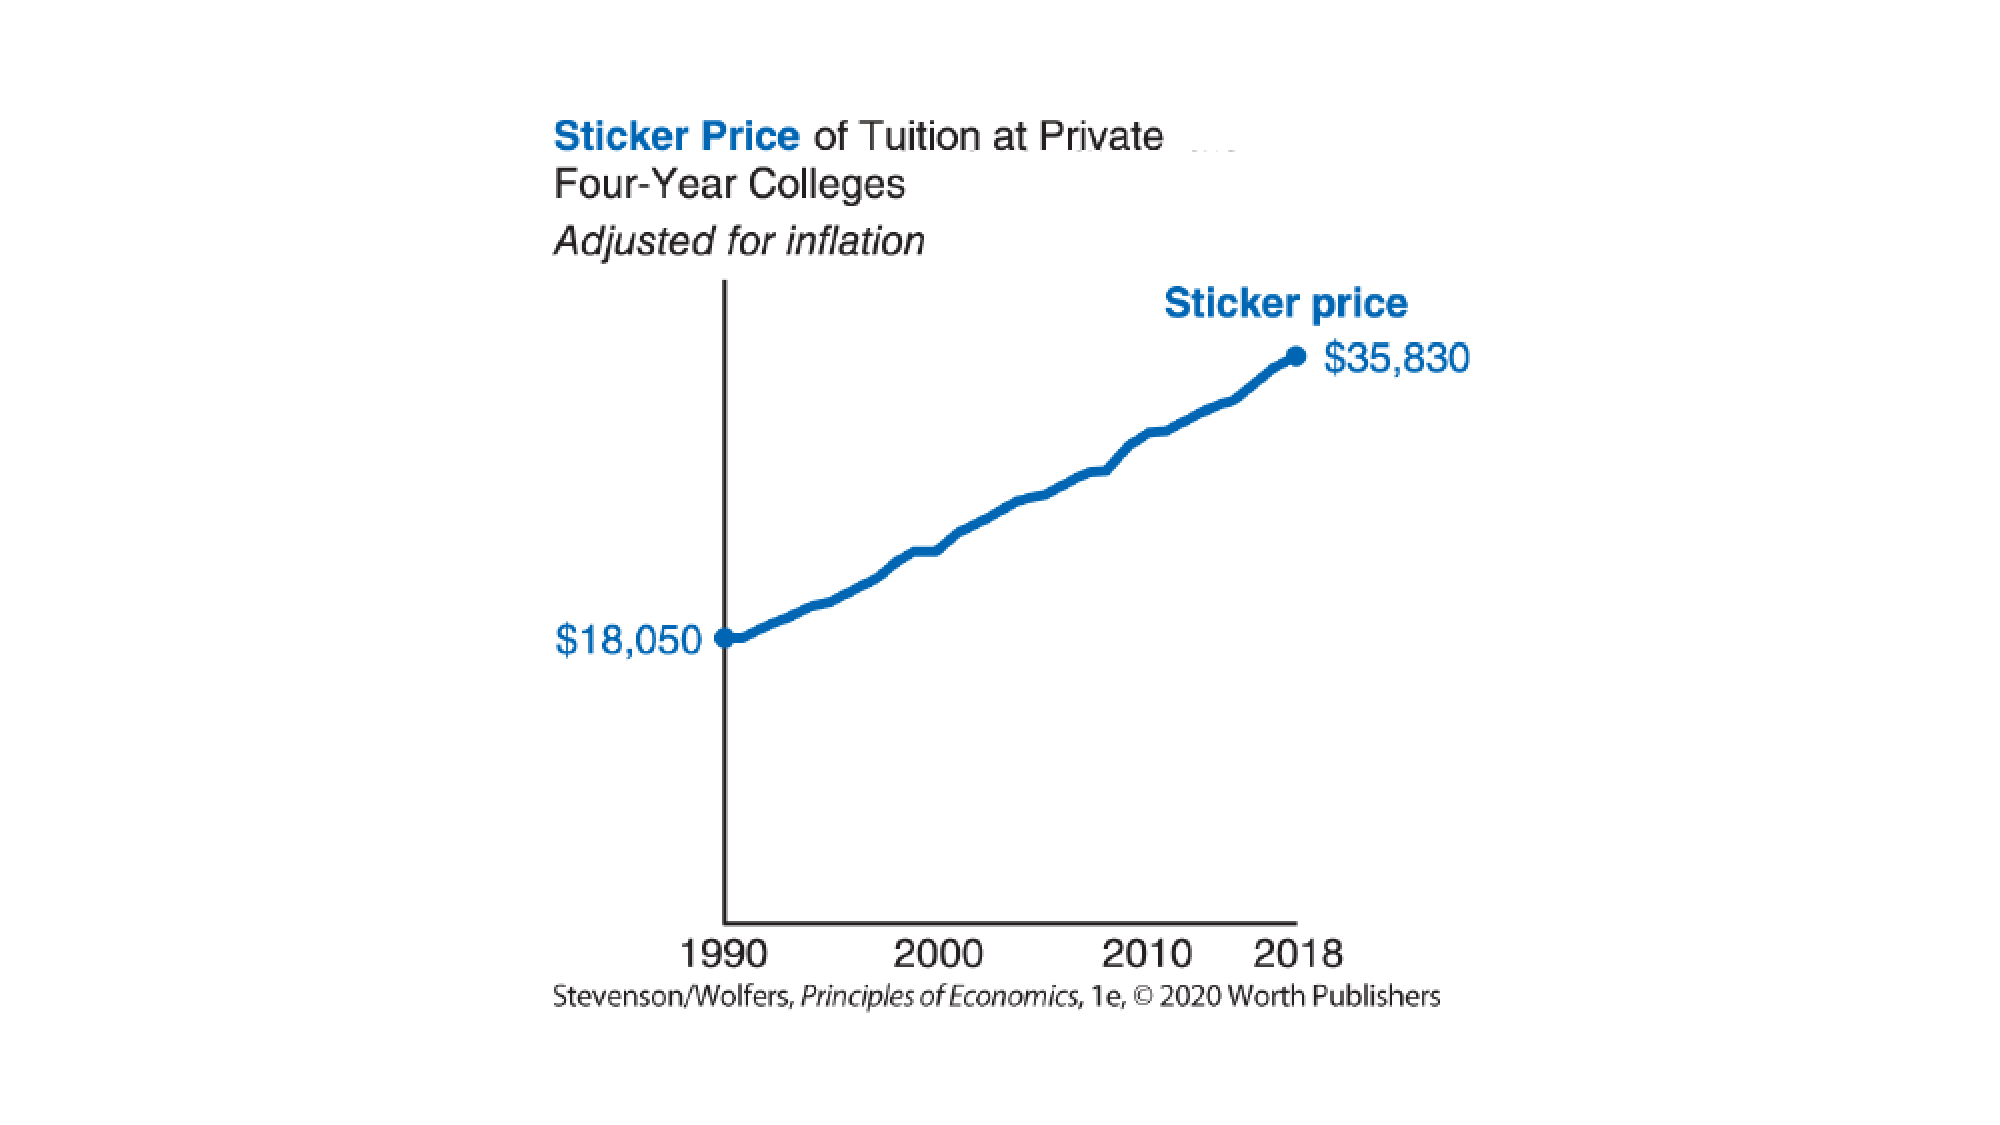
\includegraphics[width=1.0\linewidth]{college_intro}
		\caption{The Cost of Higher (Private) Education in the US, 1990 - 2018 \\ 
			\label{fig:nopd}}
 \end{figure}

	
\end{frame}
%------------------------------------------------

%\begin{frame} 
%	\frametitle{Poll}
	
%\begin{center}
%	\textbf{Trends in the cost of college since 1990 suggest... }
%\end{center}	

	
%\begin{enumerate}%[label=(\Alph*)]
%	\item A prevalent student debt problem
%	\item Benefits of Price Discrimination 
%	\item Imperfect competition in the Higher Ed market
%	\item Rising demand for Higher Ed


%\end{enumerate}
	
%\end{frame}
%------------------------------------------------

\begin{frame} 
	\frametitle{Perfect Price Discrimination (PPD)}
	
	Up until now, we only considered uniform pricing where each firm charges customers the same price
	
	\smallskip
	$\Longrightarrow$ Relax this assumption!\\
	\bigskip
	%%classification of PD goes back to Pigou (1920)
	\textbf{Key characteristics PPD}
	\begin{enumerate}
		\item Non-uniform pricing: Charge different customers different prices
			\begin{itemize}
				\item PPD commonly referred to as 1st degree Price Discrimination (PD)
			\end{itemize}
		\item Complete Information 
			\begin{itemize}
				\item Consumers' preferences known
			\end{itemize}
		\item Conditions for PD
		\begin{itemize}
			\item Firms need market power (i.e. D downward-sloping)
			\item Prevent resales %(e.g. Sony games), otherwise end up selling large Q at low P to resellers (otherwise they will undercut you)
			\item Target each customer with optimal P %i.e. max. possible P
		\end{itemize}
	\end{enumerate}

	\bigskip
		
In what follows, assume:
\begin{itemize}
	\item MC constant
	\item No FC (implies PS=Profit)
\end{itemize}
	
\end{frame}
%------------------------------------------------

\begin{frame} 
	\frametitle{Baseline (No PD): Graphical illustration}


 \begin{figure}[H]
	\centering
	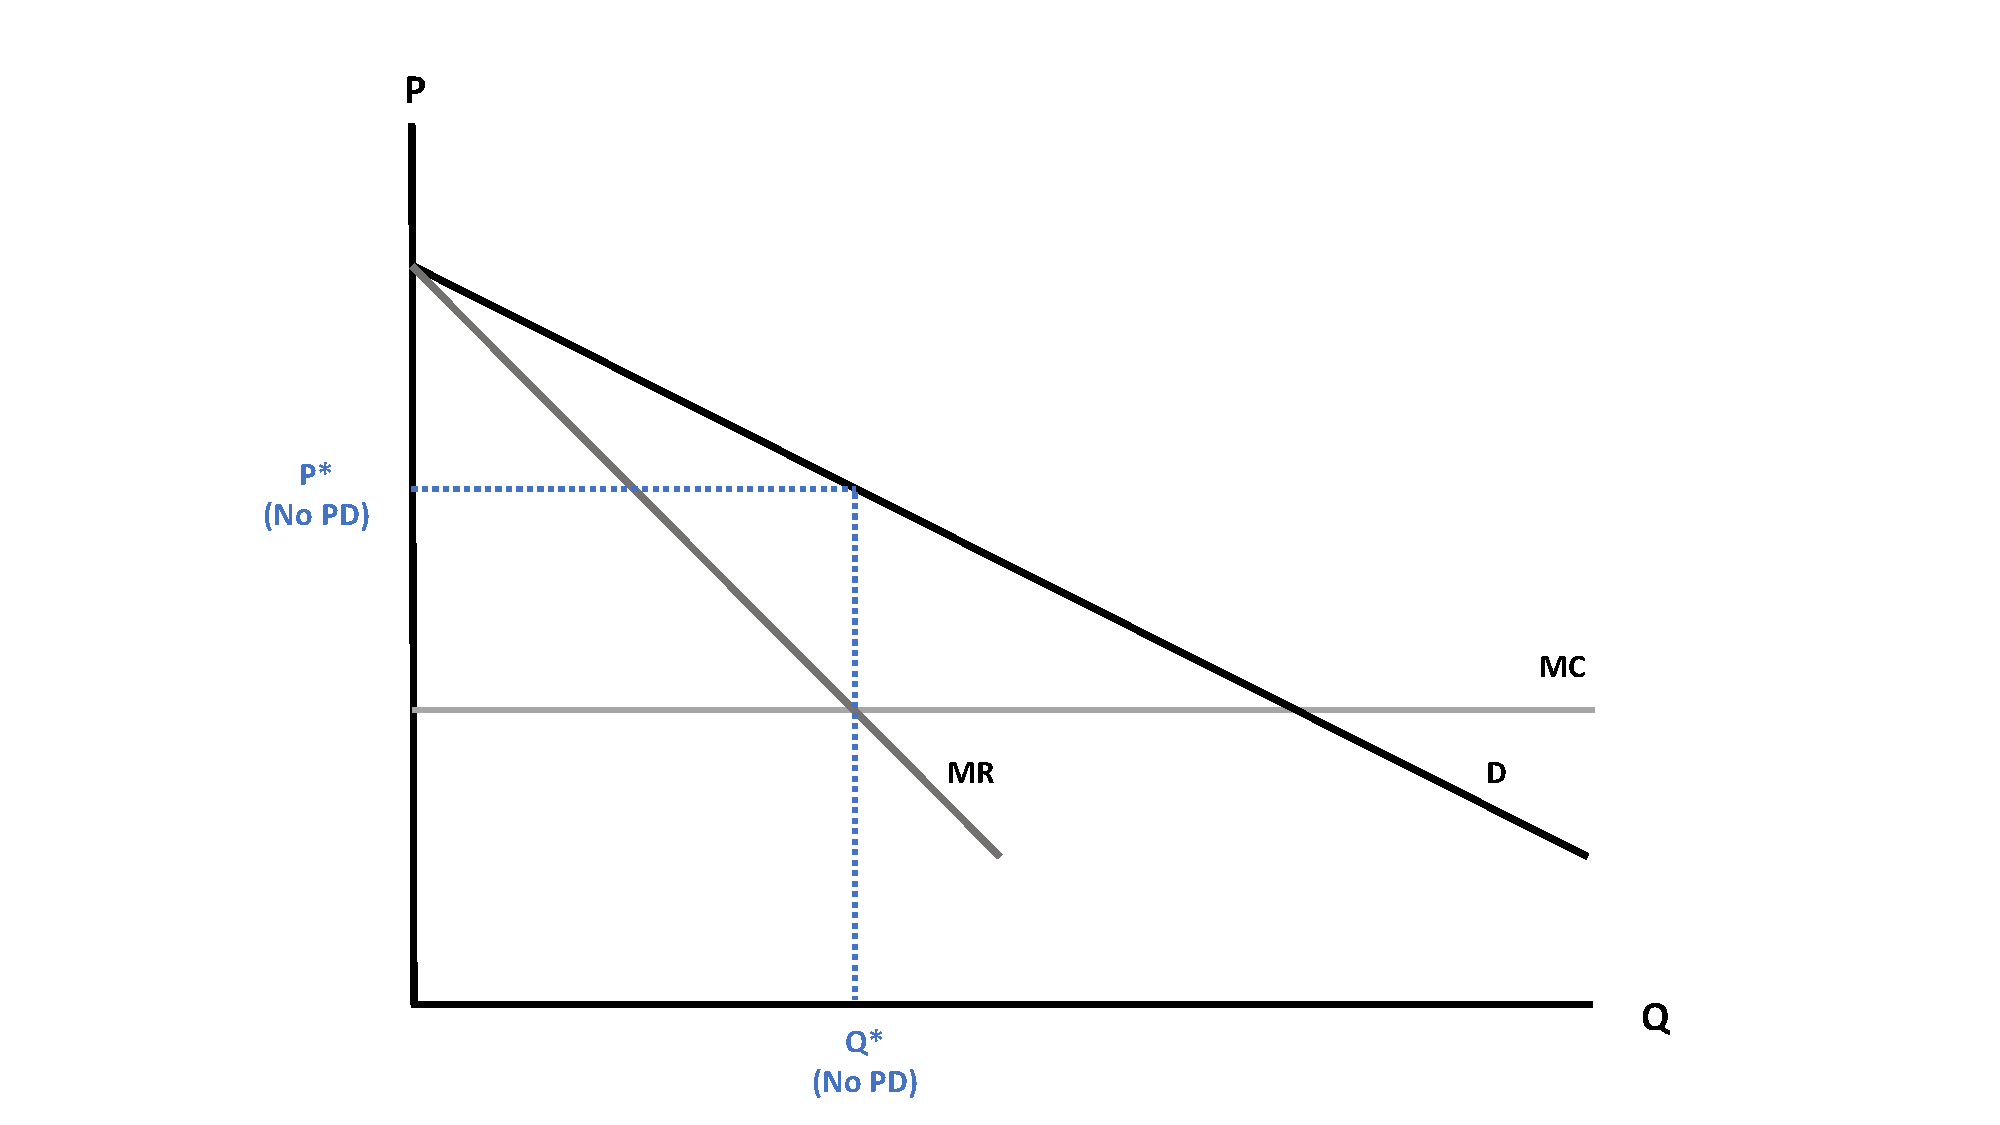
\includegraphics[width=0.8\linewidth]{no_pd}
	\caption{Monopolist: No PD \\ 
\label{fig:nopd}}

\end{figure}

\begin{itemize}
	\item Optimality: MR = MC
\end{itemize}


	
\end{frame}
%------------------------------------------------

\begin{frame} 
	\frametitle{PPD: Graphical illustration}
	
	
	\begin{figure}[H]
		\centering
		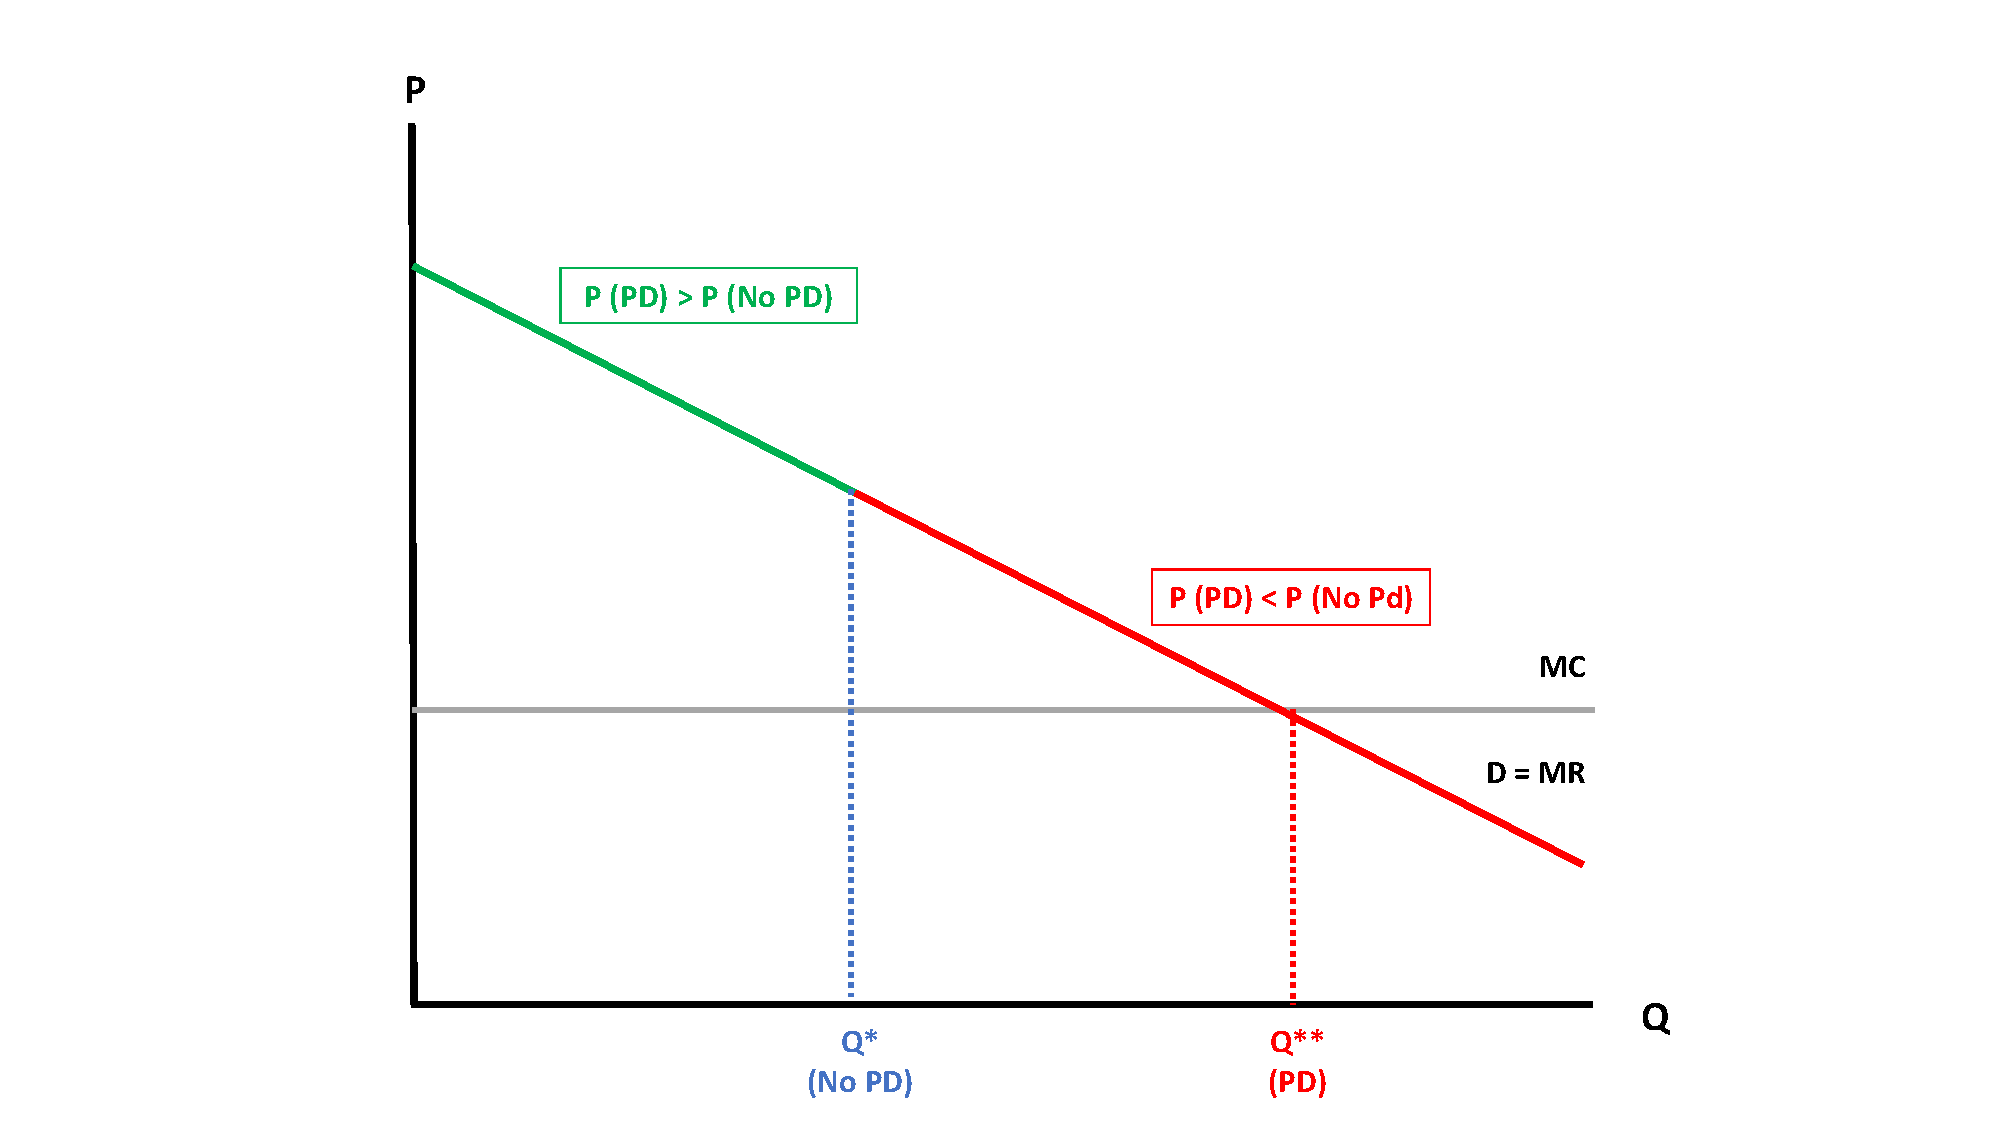
\includegraphics[width=0.8\linewidth]{pd}
		\caption{Monopolist: PPD \\ 
			\label{fig:ppd}}
		
	\end{figure}
	
	\begin{itemize}
		\item Optimality: MR = MC, P=MC
	\end{itemize}
	

\end{frame}
%------------------------------------------------

\begin{frame} 
	\frametitle{Poll}
	
	\begin{center}
		\textbf{What are the welfare implications of PPD?}
	\end{center}	
	
	\begin{enumerate}[(A)]
	\item Welfare-enhancing due to to higher output
	\item Welfare-reducing due to reduction in CS
	\item Welfare unchanged, TS simply redistributed 
\end{enumerate}

		
\end{frame}
%------------------------------------------------

\begin{frame} 
	\frametitle{Baseline (No PD): Welfare}
	

	\begin{figure}[H]
		\centering
		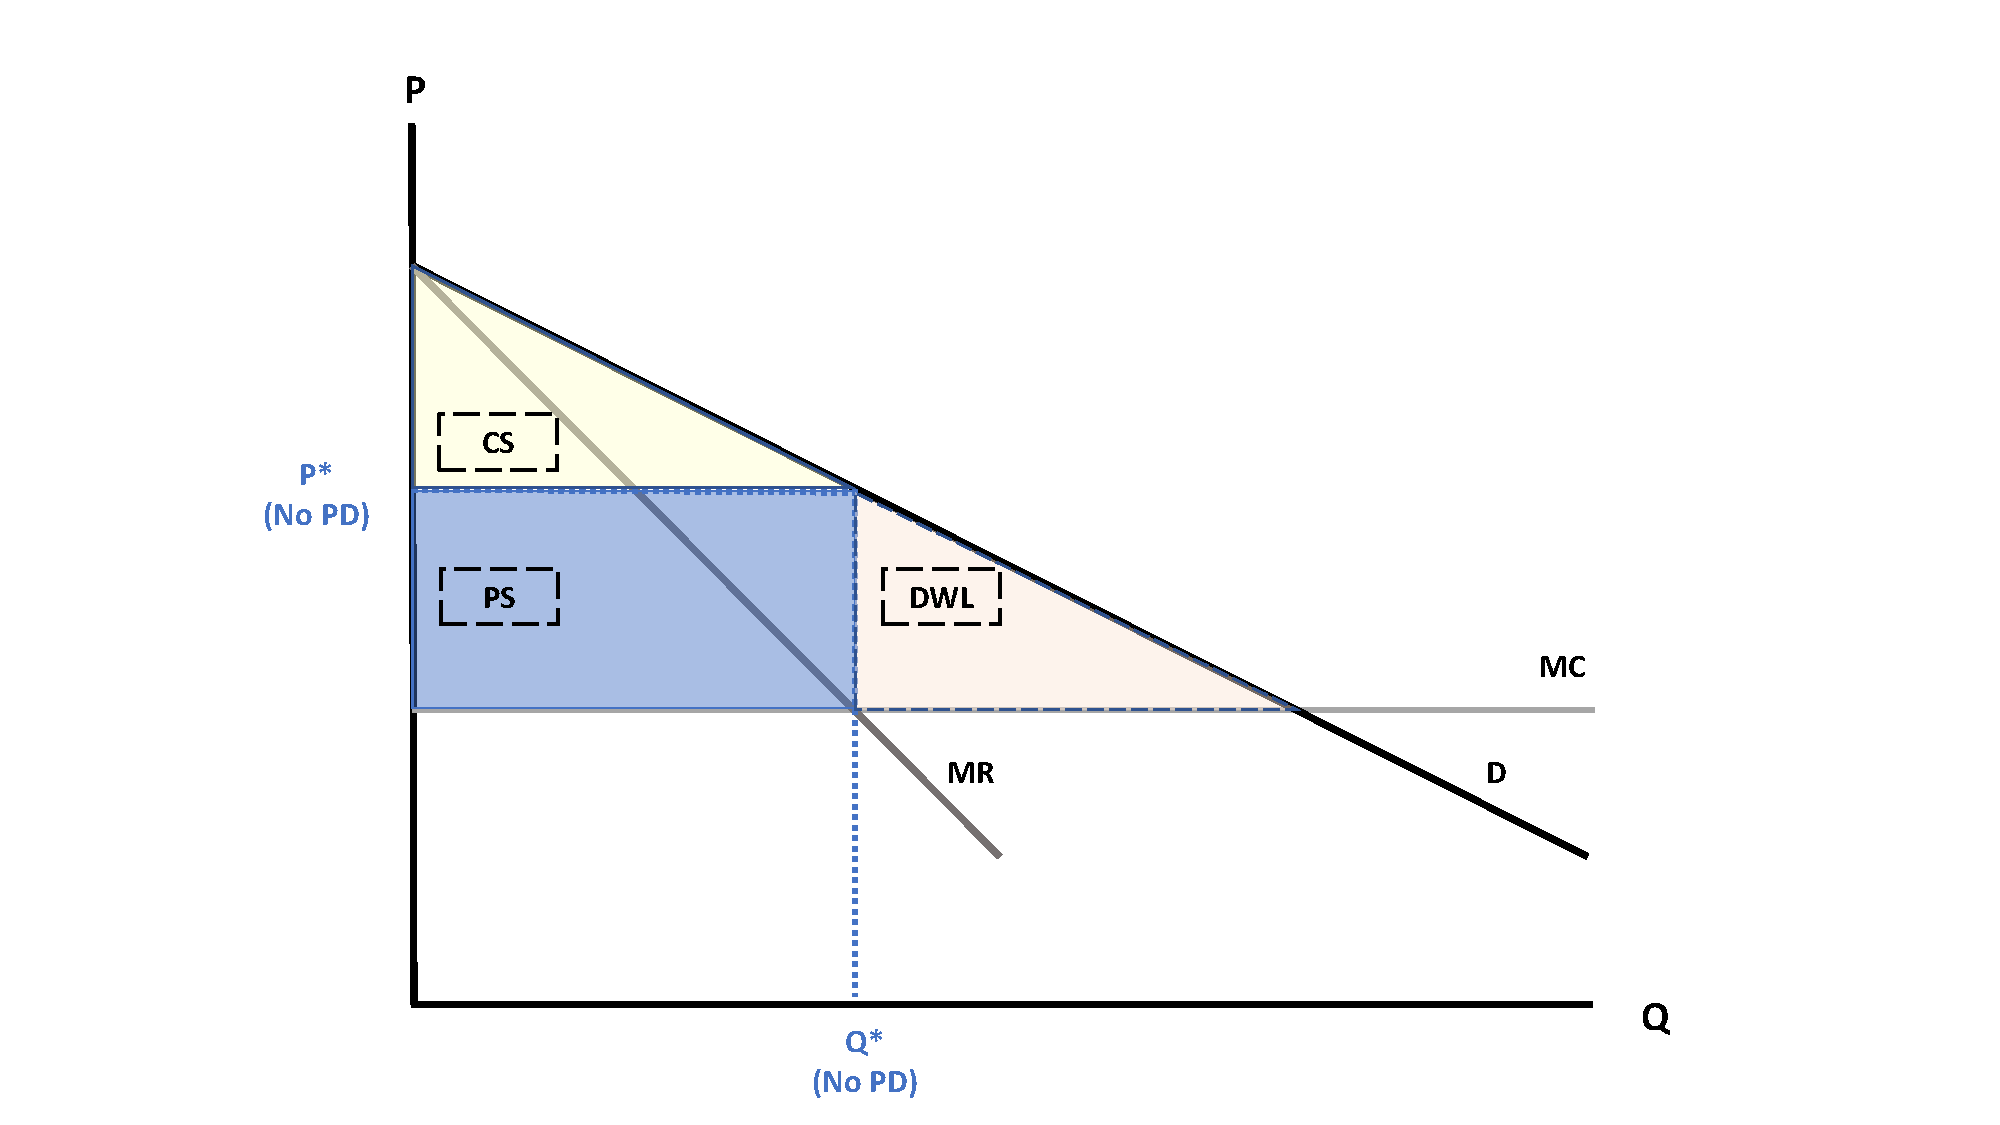
\includegraphics[width=0.78\linewidth]{no_pd_welf}
		\caption{Monopolist: No PD \\ 
			\label{fig:ppd}}
		
	\end{figure}
	
	\begin{itemize}
		\item Welfare: $\underbrace{\int_{0}^{Q*} (D - C) \,dQ}_\text{TS} = \underbrace{\int_{0}^{Q*} (D - P(Q)) \,dQ}_\text{CS} + \underbrace{\int_{0}^{Q*} (P(Q) - C)\,dQ }_\text{PS}$
	\end{itemize}
	
	
\end{frame}
%------------------------------------------------

\begin{frame} 
	\frametitle{PPD: Welfare}
	
	
	\begin{figure}[H]
		\centering
		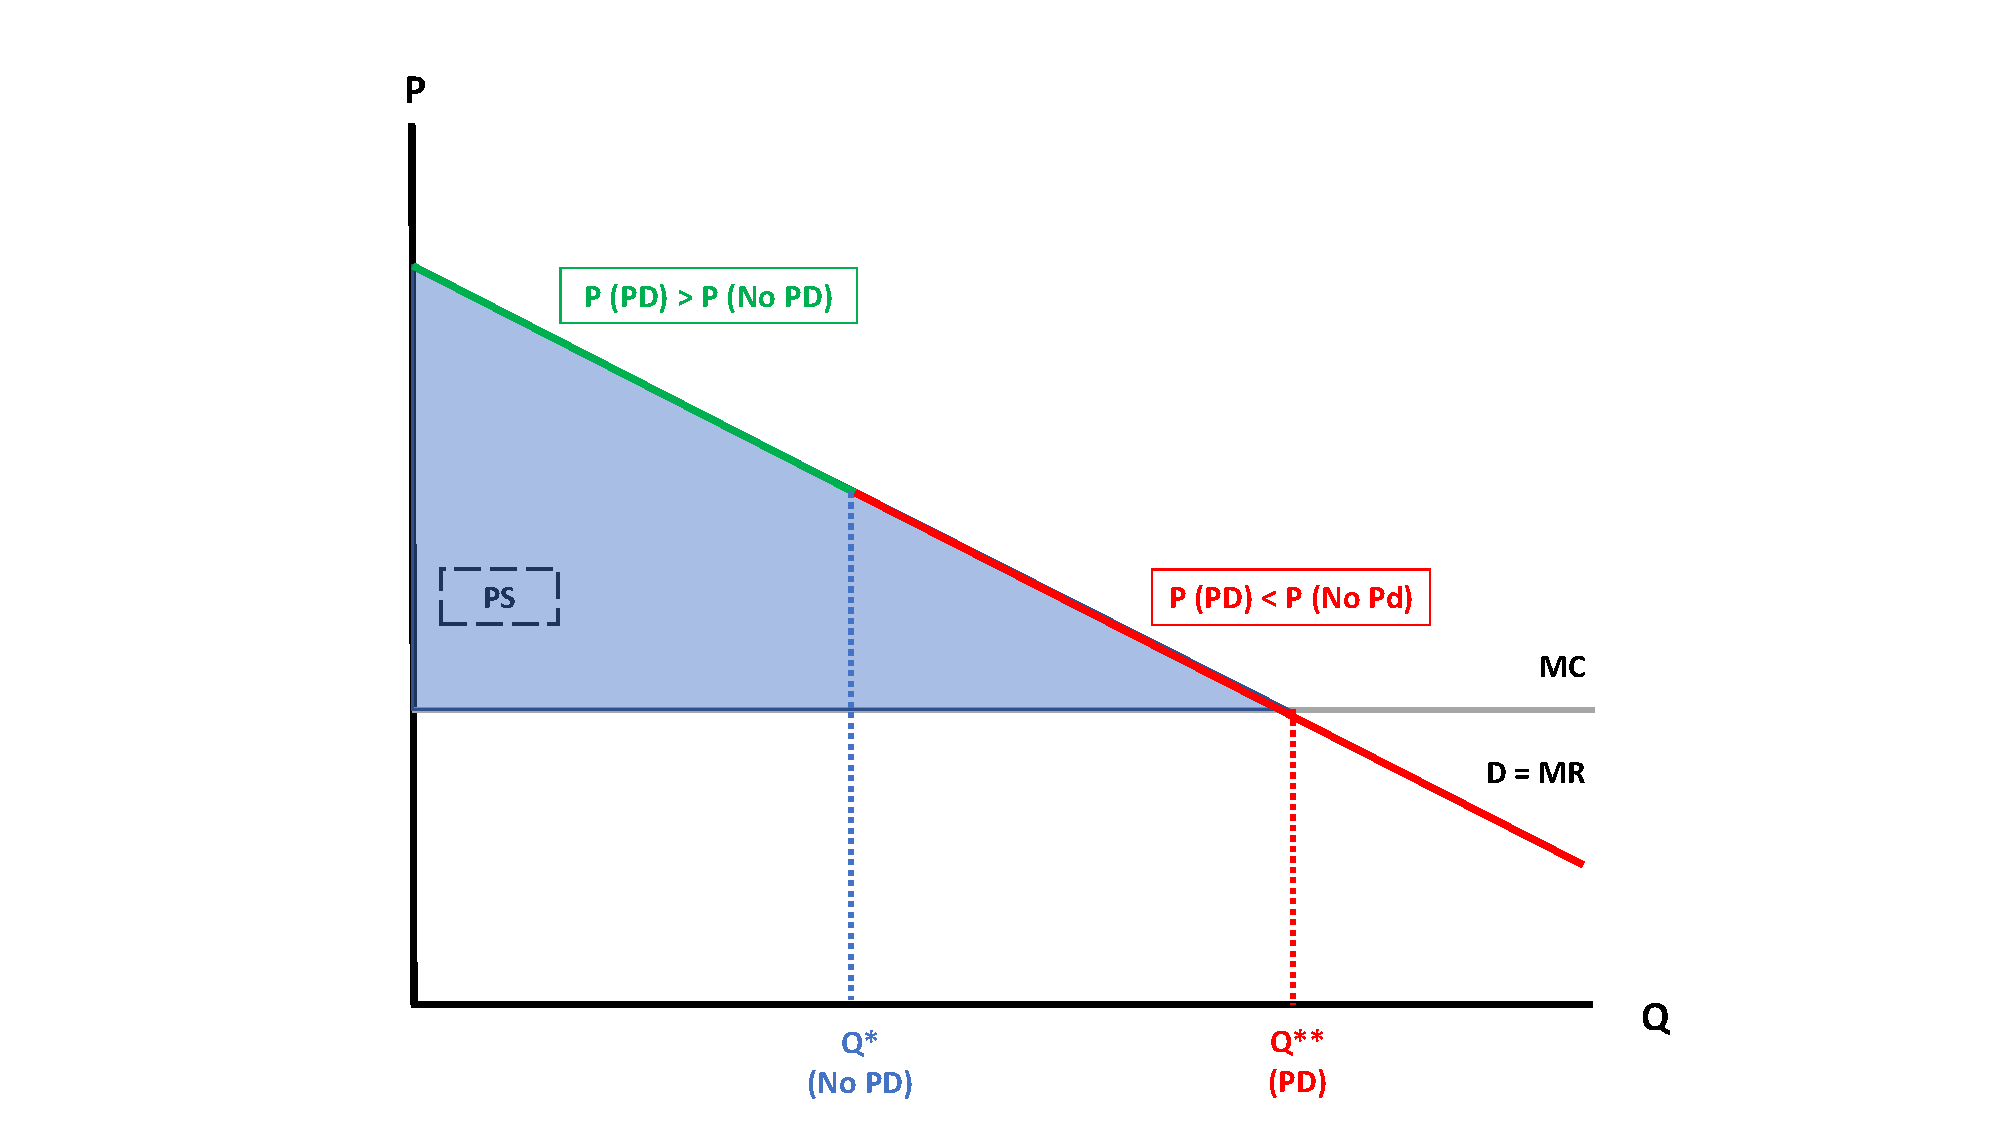
\includegraphics[width=0.78\linewidth]{pd_welf}
		\caption{Monopolist: PPD \\ 
			\label{fig:ppd}}
		
	\end{figure}
	
	\begin{itemize}
	\item Welfare: $\underbrace{\int_{0}^{Q*} (D - C) \,dQ}_\text{TS} = \underbrace{\int_{0}^{Q**} (P(Q) - C)\,dQ }_\text{PS}$
\end{itemize}
	
	
\end{frame}
%------------------------------------------------

\begin{frame} 
	\frametitle{Poll}
	
	\begin{center}
		\textbf{How do recent technological advancements in Big Data affect PD?}
	\end{center}	
	
	\begin{enumerate}[(A)]
	\item Give firms more information about your preferences
	\item Allow firms to set optimal prices
	\item Discriminate between online and offline prices
	\item Make PPD fully practical
\end{enumerate}
	
	
\end{frame}
%------------------------------------------------

\begin{frame} 
	\frametitle{PPD Application: Big Data}
	
		
	\textbf{Technological Innovations}
	
	\begin{itemize}
		\item Does Big Data lead to Price Discrimination?
		\begin{itemize}
			\item Personalization technologies (e.g., Cookies on the Web)
			\item Access to credit history, earnings profile, ...
			\item Social Media 
		\end{itemize}
		\item Price discrimination based on web browsing increases profits by 12.2\% compared to demographic information with 0.8\% (Shiller 2014)
		\item However, technology appears not advanced enough yet to make PPD fully practical
		\begin{itemize}
			\item Up to 30\% of firms' pricing decision do not deliver optimal price (Baker, Kiewll \& Winkler 2014)
			\item Prices collected online and offline are identical in 72\% of cases (Cavallo 2017)
		\end{itemize}
		\item Other related factors preventing PPD are managerial inertia and concerns about brand image (DellaVigna \& Gentzkow 2019)
	\end{itemize}
	
	\bigskip
\textbf{Is PPD feasible?} 

\begin{itemize}
	\item Key problem: Incomplete Information
	\begin{itemize}
		\item [$\Longrightarrow$] Do not observe consumer's reservation price
	\end{itemize}
\end{itemize}	
	
\end{frame}
%------------------------------------------------


\begin{frame} 
	\frametitle{PD: Non-linear pricing (2nd degree PD)}
	
%	\begin{figure}[H]
%	\centering
%	
\includegraphics[width=0.2\linewidth]{edeka}
%	\caption{Monopolist: PPD \\ 
%		\label{fig:ppd}}
	
%\end{figure}

%	\textbf{Is PPD feasible?} 

%\begin{itemize}
%	\item Key problem: Incomplete Information
%	\begin{itemize}
%		\item [$\Longrightarrow$] Do not observe consumer's reservation price
%	\end{itemize}
%\end{itemize}

%\bigskip

	\begin{itemize}
		
		\item 2PD relies on various forms of self-selection
		\smallskip
			\begin{itemize}
				\item Quantity Targeting (``Hurdle method '')
					\begin{itemize}
						\item Quantity discounts (``2 for 1'')
						\item Bundling (Package deals)%people who bough this item also purchased --- water filtration system, also get a set of water filters
					\end{itemize}
				\item Quality Targeting 
					\begin{itemize}
						\item Flying Economy (E) vs. First-Class (FC)
					\end{itemize}
				
			\end{itemize}	

	\end{itemize}
\bigskip

\textbf{\begin{center} Example: \\Discriminate between Business Travelers (B) \& Tourists (T) \end{center}} 
\begin{itemize}
	\item (i) Individual rationality constraints (Participation)%buy plane ticket
	\begin{itemize}
		\item $u_{FC}^{B} - P_{FC} > 0$
		\item $u_{E}^{T} - P_{E} > 0$
	\end{itemize}
	\item (ii) Incentive-compatibility constraints (Self-selection)%buy approp. seat based on your WTP
		\begin{itemize}
		\item $u_{FC}^{B} - P_{FC} > u_{E}^{B} - P_{E}$
		\item $u_{E}^{T} - P_{E} > u_{FC}^{T} - P_{FC}$
	\end{itemize}

	
%		\begin{itemize}
%			\item 3PD leads to higher output, yet, net effects depend on degree of misallocation in response to redistribution of CS
%		\end{itemize}

\end{itemize}
%Bundling: combining goods with high and low MB (Word, Excel / Cable TV)
	
%	Why are firms so creative with various non-linear pricing schemes under 2nd degree PD? Cannot classify customers into groups
	
%	Example: Ex ante airlines cannot differentiate between business travellers and tourists - Solution? Let them tell us!
	

	
\end{frame}
%------------------------------------------------

\begin{frame} 
	\frametitle{PD: Group-specific pricing (3rd degree PD)}
	
\begin{itemize}
		\item Welfare under 2PD lower than PPD %inherent to any sort of self-selection problem where you depend on revealed preferences/ signals (might be too much noise for credible information)
		\begin{itemize}
			\item Challenging to identify different types of consumers (despite Big Data)
			\item 2PD requires lots of detailed information on customers 
		\end{itemize}
		
	\begin{itemize}
		\item [$\Longrightarrow$] Not always feasible or practical
	\end{itemize}
\end{itemize}

%2pd more difficult, both for us to analyze and for the seller to pull off, than it is for 1st or 3rd degree because here types or WTP are not observable.
%so, seller must rely on self­selection, but how could that possibly work because consumers will not willingly pay more just because their (unobserved) WTP is higher

\bigskip

\textbf{More convenient strategy:}
	
	\begin{itemize}
		
		\item Group pricing 
		\begin{itemize}
			\item 3PD relies on broad market segmentation
				\begin{itemize}
					\item Student/ Seniority discounts
					\item New Customer Bonus (``Teaser'')%gym fees
					\item Geographic discrimination%textbooks more expensive in affluent parts of the world
				\end{itemize}
			\item Group-specific optimization
		\end{itemize}
	\end{itemize}
	

	
\end{frame}
%------------------------------------------------

\begin{frame} 
	\frametitle{PD: Group-specific pricing (3rd degree PD)}


\begin{figure}[H]
	\centering
	\begin{subfigure}[]{0.49\textwidth}
		\centering
		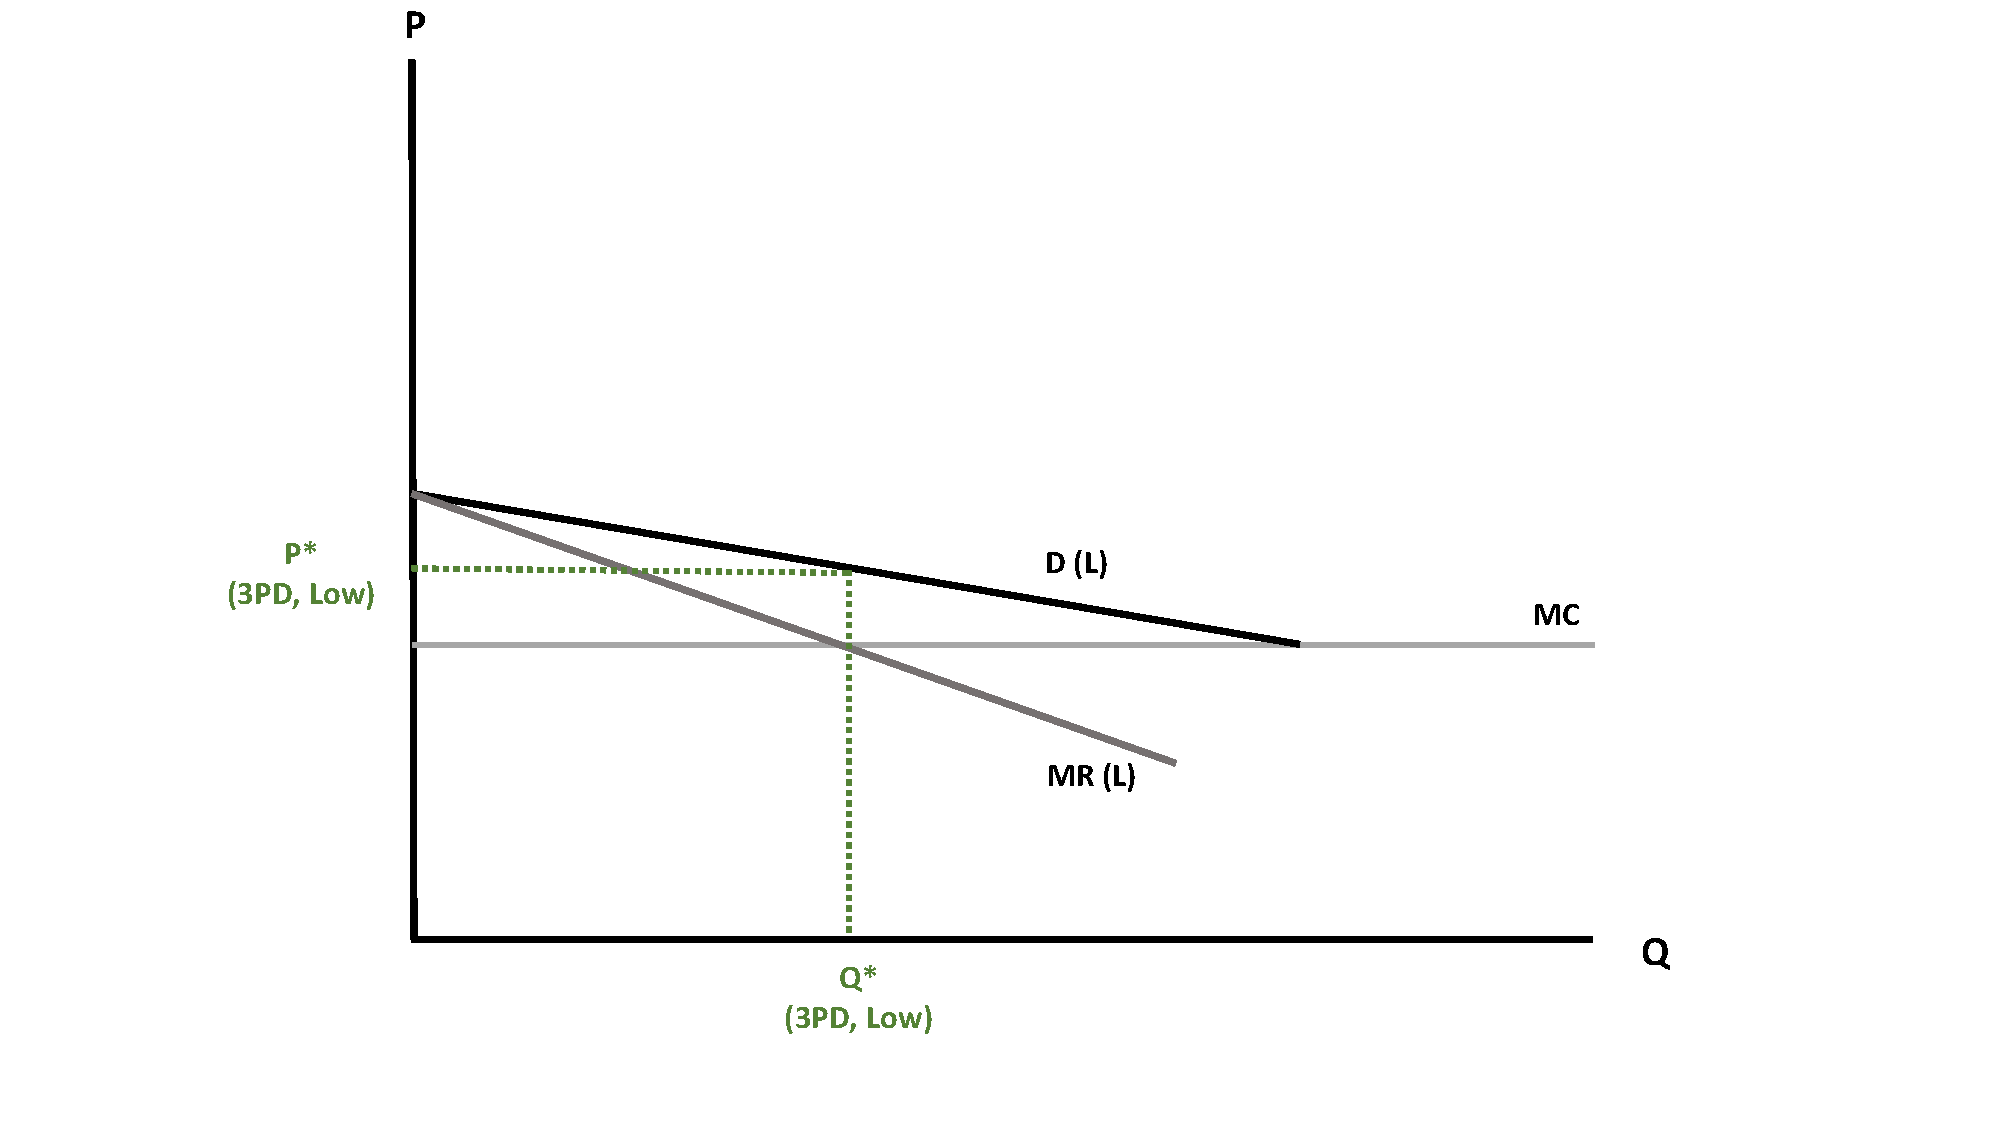
\includegraphics[width=\linewidth]{3pd_low.pdf} 
		\caption{Students (L)} \label{fig:stud}
	\end{subfigure}
	\hfill
	\begin{subfigure}[]{0.49\textwidth}
		\centering
		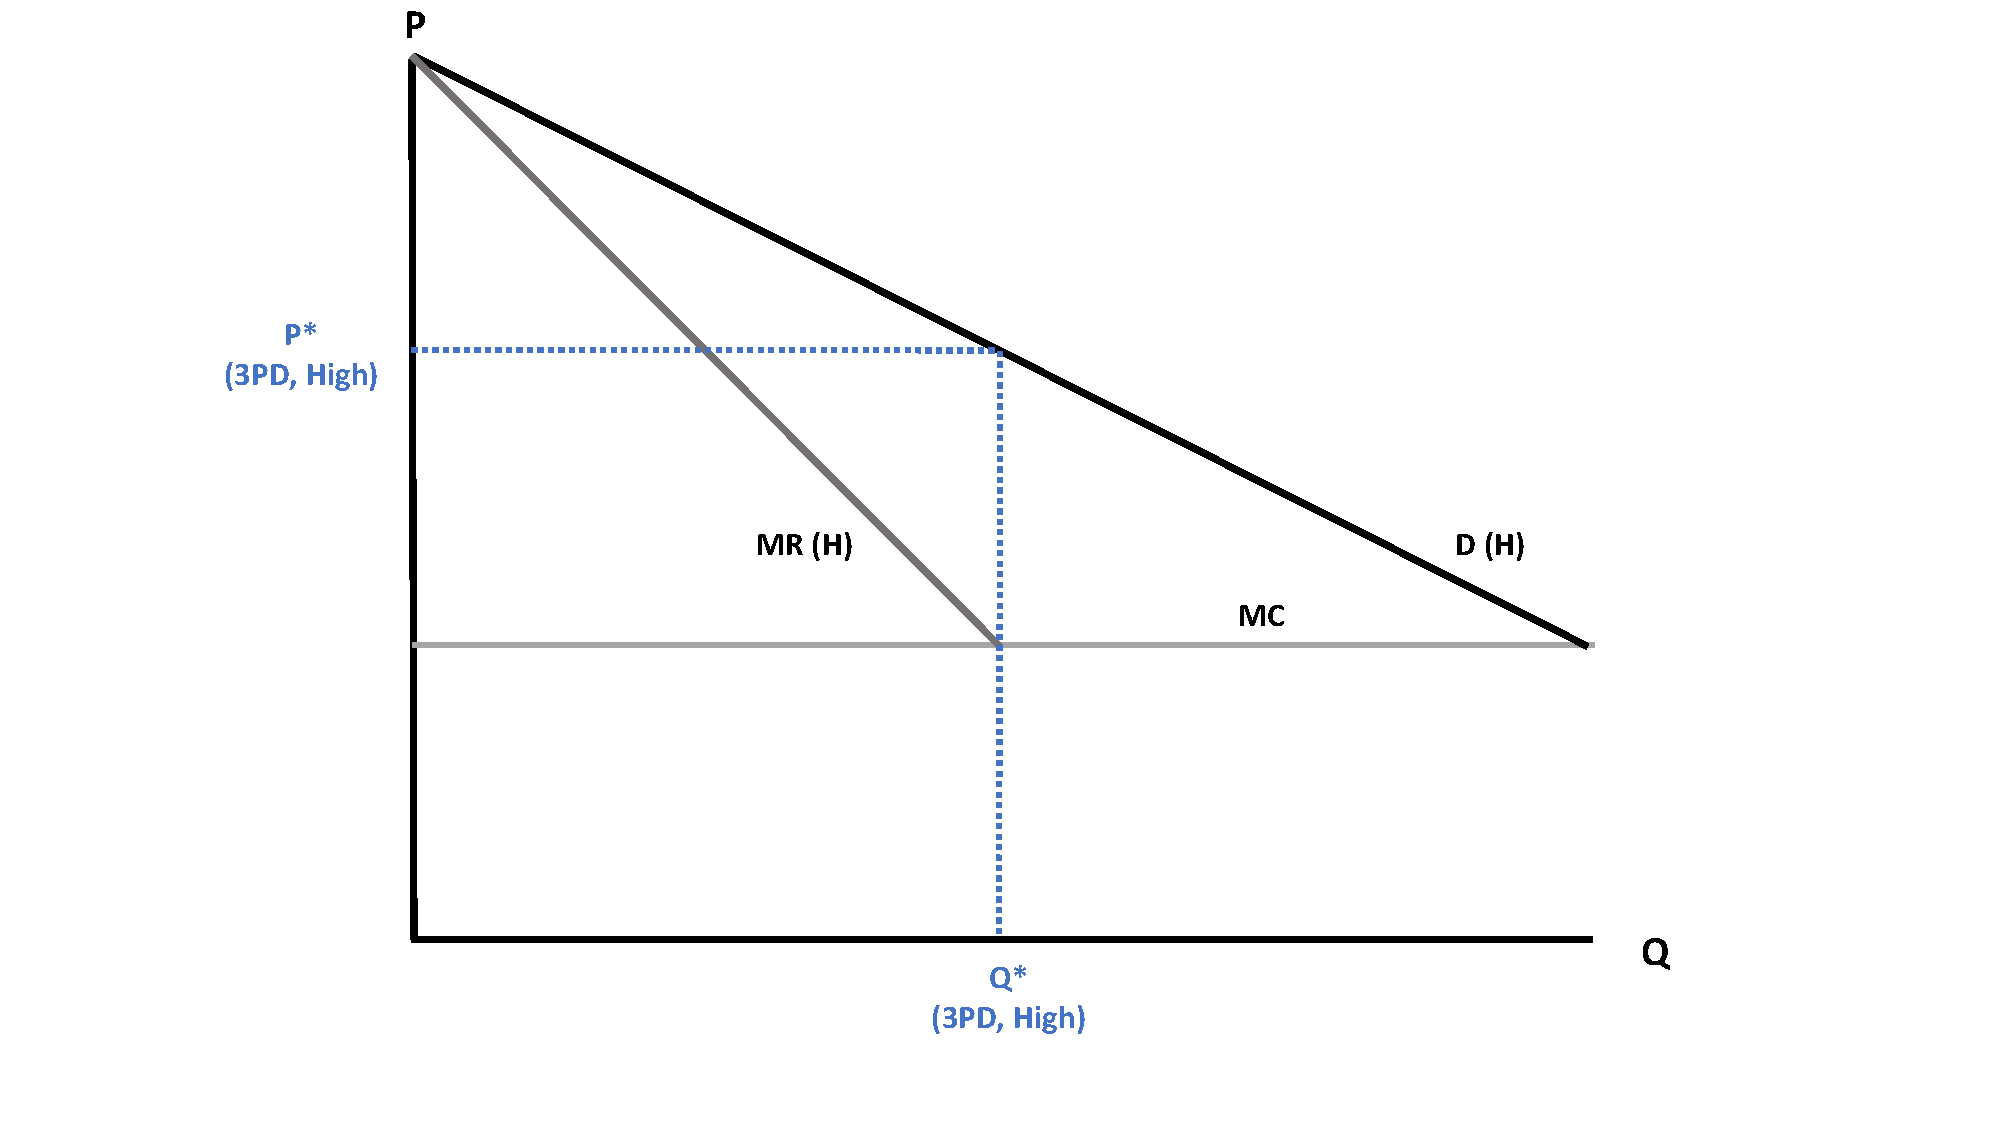
\includegraphics[width=\linewidth]{3pd_high.pdf} 
		\caption{Professionals (H)} \label{fig:prof}
	\end{subfigure}
	\caption{Price Discrimination for Economic Conferences}
\end{figure}


%% D for students lower due to more binding BCs & flatter as their D is more elastic, i.e. more responsive to prices  --- otherwise markets are identical

\begin{itemize}
	\item Optimality requires: $MR_{H}=MR_{L}=MC$
	\item Welfare? Ambiguous! 
		\begin{itemize}
			\item 3PD leads to higher output, yet, net effects depend on degree of misallocation in response to redistribution of CS
		\end{itemize}
\end{itemize}
%welfare effects are ambiguous –DWL might be mitigated relative to uniform price if output goes up, but there is also a misallocation –some that purchase in low-price group might have lower valuation for good than a non-purchaser in the high price group.

%a necessay condition for welfare improvement is that total output has increased a sufficient condition for welfare improvement is that weighted output has increased, where the weights in each market is given by the divergence between price and marginal cost

%In words, price discrimination leads to an increase in output if the discrepancy in elasticities across the two markets is greater with respect to the outside option than with respect to the rival’s good. Among other things, this condition implies that at the discriminating monopoly prices (where the left-hand ratio is 1), the strong market is “more competitive” than the weak market in the sense of cross-price elasticities 
%--> There could be two equilibria (both markets served with uniform pricing or only high P served; in the former case there would be kinks in the D curve)If low P demand is “low enough” or MC “high enough” serve only high P group, then would do uniform pricing for high P group

%Robinson (1933) showed that the movement toward third degree discriminating prices alters the distribution of output but does not change total output when demand curves are linear. Schmalensee (1981) showed that deadweight loss increases unless output increases. Thus, when demand curves are linear, the implementation of third degree price discrimination increases deadweight loss. Ikeda and Toshimitsu (2010), using a model in which consumers have unit demand and quality is endogenous, show that an increase in total output is a necessary condition for welfare improvement with third degree price discrimination by a monopolist. T

%Thus, when output does not increase, the provision of information on customer type that allows the firm to implement third degree price discrimination lowers welfare. This conclusion, implicit in textbook treatments, is the opposite of the result presented above. The source of the divergence in the conclusion is due to the use (by the Pigouvian taxonomy) of linear pricing rather than non-linear pricing. This results in the firm reducing output to the type H customers in an attempt to capture their consumer surplus. The output supplied to type M customers however increases. This result contrasts to that obtained above for non-linear pricing, where output supplied to type M customers decreases due to implementation of price discrimination. By comparison Ikeda and Toshimitsu (2010) show that third degree price discrimination always enhances welfare when quality is endogenous, mainly because of the quality improvement owing to price discrimination increases consumer surplus.

%Thus the conclusions derived from the textbook analysis of (Pigouvian) third degree price discrimination follows from the joint assumptions of linear pricing (i.e. intra-group arbitrage but no inter-group arbitrage) and the availability of an exogenous signal on customer types (or groups of types). The above analysis can be readily extended to the case of three customer types. In this event, as with non-linear pricing there are three possibilities:
%(i) pure direct linear pricing in which each type faces their own linear price;
%(ii) partial direct linear pricing in which the firm observes an exogenous signal about one type (which we take to be type L) and cannot distinguish between the other two types (H and M): in this case the firm charges one linear price to the type with the exogenous signal (type L) and a common price to the types that cannot be separated (H and M); and
%(iii) common linear pricing in which the firm cannot distinguish between all threecustomer types.
\end{frame}
%------------------------------------------------

\begin{frame} 
	\frametitle{Motivational Example Revisited}
	
	
	\begin{figure}[H]
		\centering
		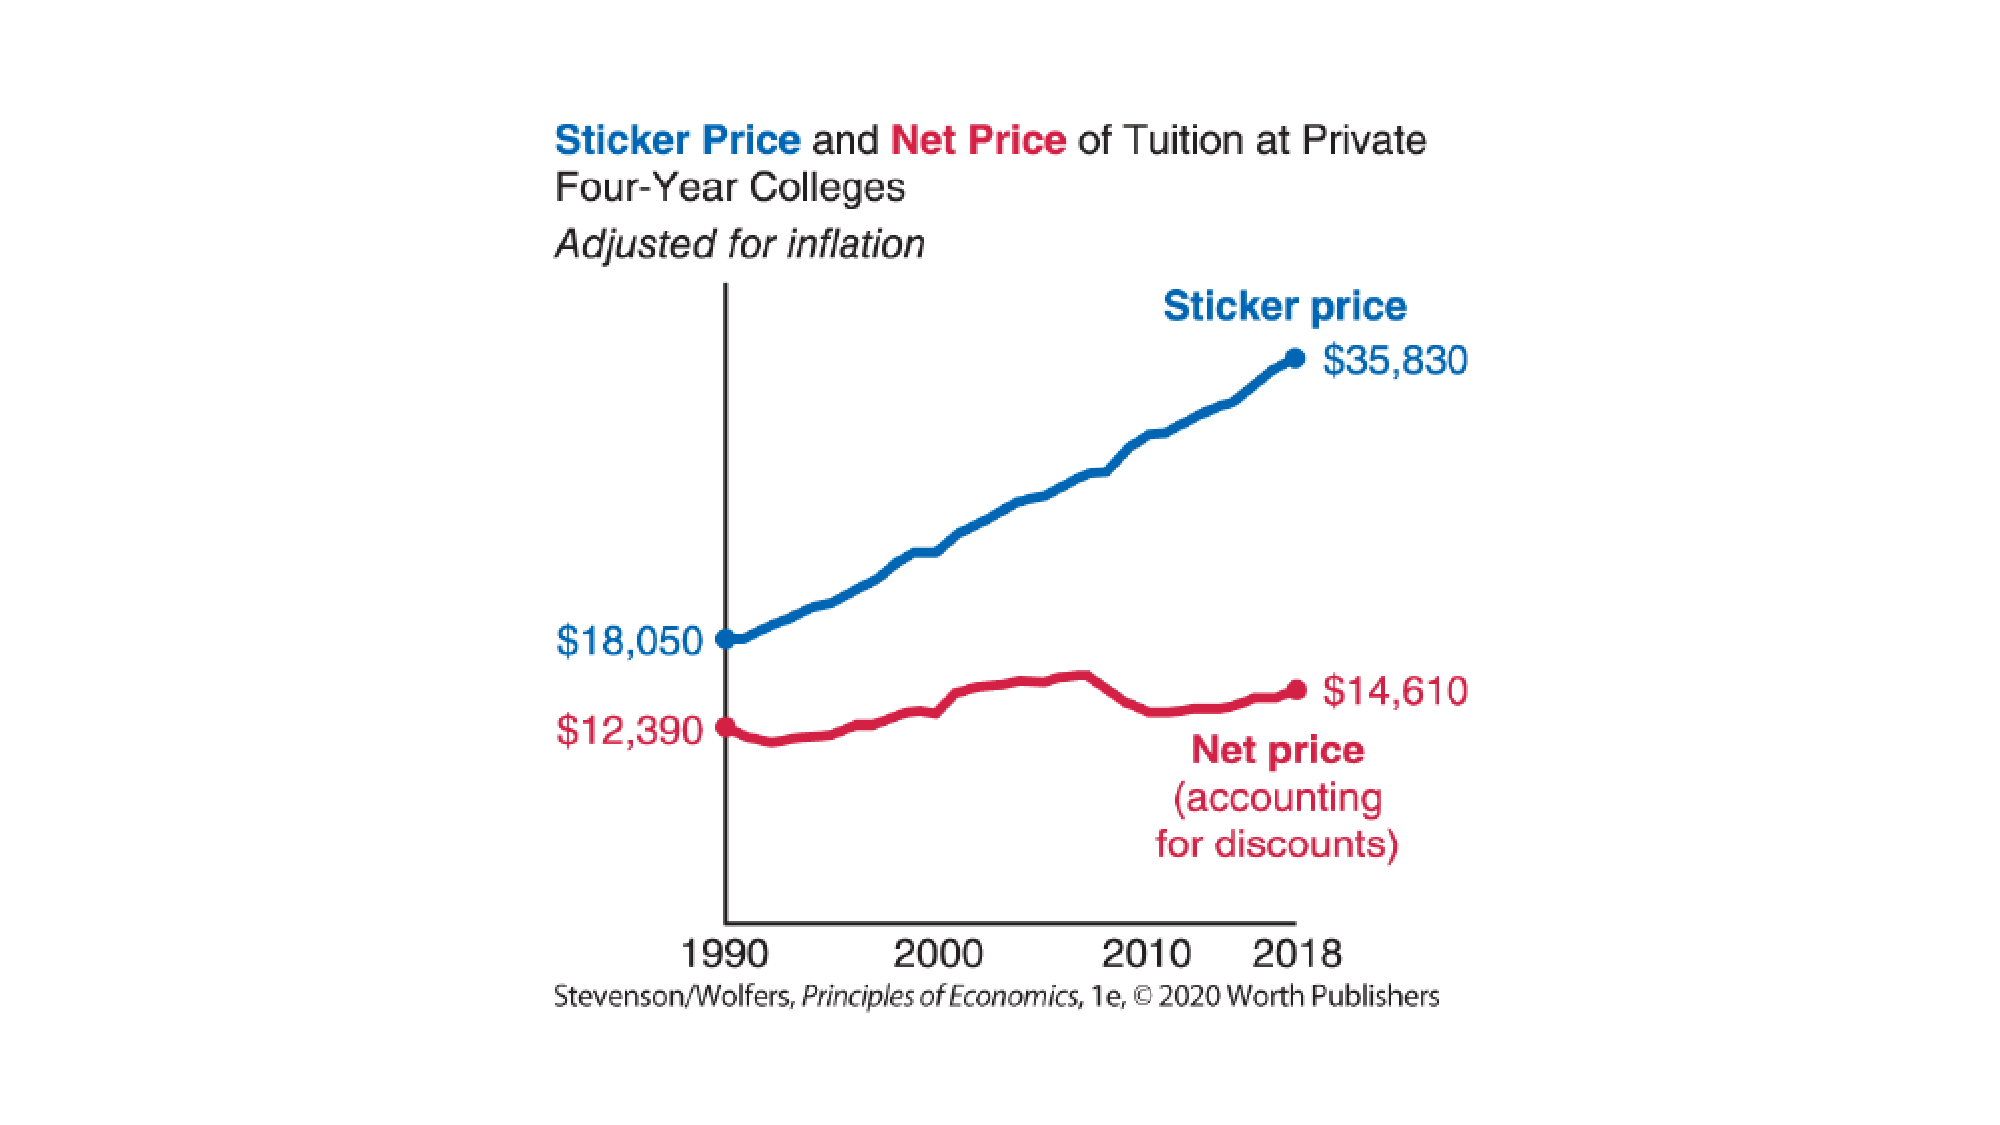
\includegraphics[width=1.0\linewidth]{college_pd}
		\caption{Price Discrimination in Higher (Private) Education in the US, 1990 - 2018 \\ 
			\label{fig:nopd}}
	\end{figure}
	

\end{frame}
%------------------------------------------------

\end{document}